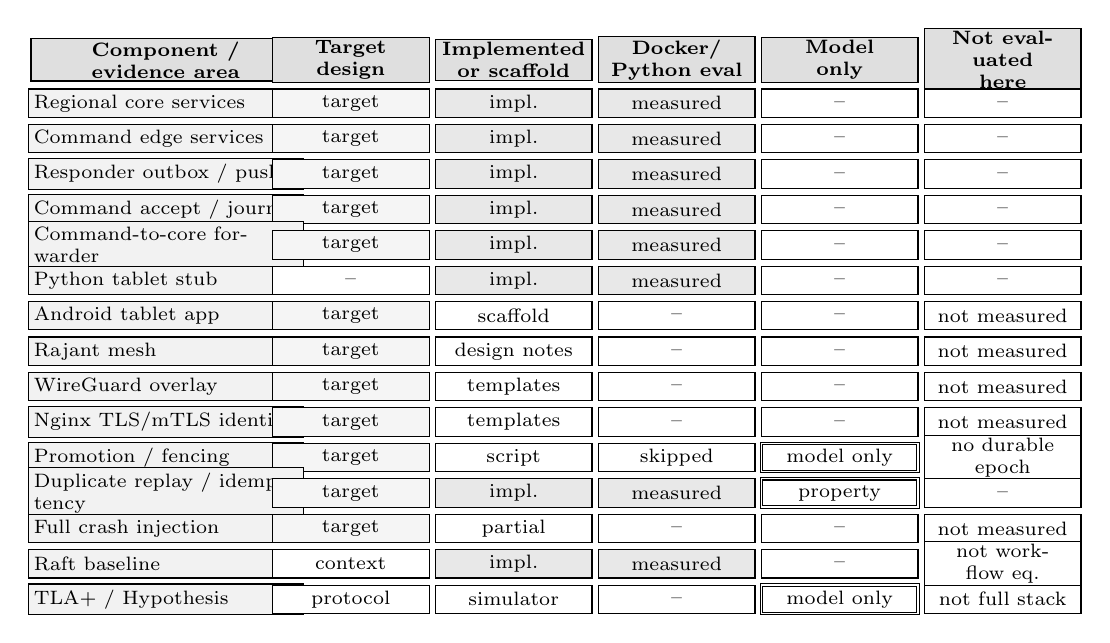
\begin{tikzpicture}[
  x=1cm,y=1cm,
  component/.style={draw, fill=gray!10, font=\scriptsize, align=left, text width=3.35cm, minimum height=0.36cm, inner sep=2pt},
  head/.style={draw, fill=gray!25, font=\scriptsize\bfseries, align=center, text width=1.92cm, minimum height=0.52cm, inner sep=1pt},
  chead/.style={head, text width=3.35cm},
  cell/.style={draw, font=\scriptsize, align=center, text width=1.92cm, minimum height=0.36cm, inner sep=1pt},
  measured/.style={cell, fill=gray!18},
  target/.style={cell, fill=gray!8},
  scaffold/.style={cell, fill=white},
  model/.style={cell, double, double distance=0.5pt},
  empty/.style={cell, fill=white}
]
\node[chead] at (1.70,0) {Component / evidence area};
\node[head]  at (4.05,0) {Target\\design};
\node[head]  at (6.12,0) {Implemented\\or scaffold};
\node[head]  at (8.19,0) {Docker/\\Python eval};
\node[head]  at (10.26,0) {Model\\only};
\node[head]  at (12.33,0) {Not evaluated\\here};

\node[component] at (1.70,-0.55) {Regional core services};
\node[target]    at (4.05,-0.55) {target};
\node[measured]  at (6.12,-0.55) {impl.};
\node[measured]  at (8.19,-0.55) {measured};
\node[empty]     at (10.26,-0.55) {--};
\node[empty]     at (12.33,-0.55) {--};

\node[component] at (1.70,-1.00) {Command edge services};
\node[target]    at (4.05,-1.00) {target};
\node[measured]  at (6.12,-1.00) {impl.};
\node[measured]  at (8.19,-1.00) {measured};
\node[empty]     at (10.26,-1.00) {--};
\node[empty]     at (12.33,-1.00) {--};

\node[component] at (1.70,-1.45) {Responder outbox / push};
\node[target]    at (4.05,-1.45) {target};
\node[measured]  at (6.12,-1.45) {impl.};
\node[measured]  at (8.19,-1.45) {measured};
\node[empty]     at (10.26,-1.45) {--};
\node[empty]     at (12.33,-1.45) {--};

\node[component] at (1.70,-1.90) {Command accept / journal};
\node[target]    at (4.05,-1.90) {target};
\node[measured]  at (6.12,-1.90) {impl.};
\node[measured]  at (8.19,-1.90) {measured};
\node[empty]     at (10.26,-1.90) {--};
\node[empty]     at (12.33,-1.90) {--};

\node[component] at (1.70,-2.35) {Command-to-core forwarder};
\node[target]    at (4.05,-2.35) {target};
\node[measured]  at (6.12,-2.35) {impl.};
\node[measured]  at (8.19,-2.35) {measured};
\node[empty]     at (10.26,-2.35) {--};
\node[empty]     at (12.33,-2.35) {--};

\node[component] at (1.70,-2.80) {Python tablet stub};
\node[empty]     at (4.05,-2.80) {--};
\node[measured]  at (6.12,-2.80) {impl.};
\node[measured]  at (8.19,-2.80) {measured};
\node[empty]     at (10.26,-2.80) {--};
\node[empty]     at (12.33,-2.80) {--};

\node[component] at (1.70,-3.25) {Android tablet app};
\node[target]    at (4.05,-3.25) {target};
\node[scaffold]  at (6.12,-3.25) {scaffold};
\node[empty]     at (8.19,-3.25) {--};
\node[empty]     at (10.26,-3.25) {--};
\node[scaffold]  at (12.33,-3.25) {not measured};

\node[component] at (1.70,-3.70) {Rajant mesh};
\node[target]    at (4.05,-3.70) {target};
\node[scaffold]  at (6.12,-3.70) {design notes};
\node[empty]     at (8.19,-3.70) {--};
\node[empty]     at (10.26,-3.70) {--};
\node[scaffold]  at (12.33,-3.70) {not measured};

\node[component] at (1.70,-4.15) {WireGuard overlay};
\node[target]    at (4.05,-4.15) {target};
\node[scaffold]  at (6.12,-4.15) {templates};
\node[empty]     at (8.19,-4.15) {--};
\node[empty]     at (10.26,-4.15) {--};
\node[scaffold]  at (12.33,-4.15) {not measured};

\node[component] at (1.70,-4.60) {Nginx TLS/mTLS identity};
\node[target]    at (4.05,-4.60) {target};
\node[scaffold]  at (6.12,-4.60) {templates};
\node[empty]     at (8.19,-4.60) {--};
\node[empty]     at (10.26,-4.60) {--};
\node[scaffold]  at (12.33,-4.60) {not measured};

\node[component] at (1.70,-5.05) {Promotion / fencing};
\node[target]    at (4.05,-5.05) {target};
\node[scaffold]  at (6.12,-5.05) {script};
\node[empty]     at (8.19,-5.05) {skipped};
\node[model]     at (10.26,-5.05) {model only};
\node[scaffold]  at (12.33,-5.05) {no durable epoch};

\node[component] at (1.70,-5.50) {Duplicate replay / idempotency};
\node[target]    at (4.05,-5.50) {target};
\node[measured]  at (6.12,-5.50) {impl.};
\node[measured]  at (8.19,-5.50) {measured};
\node[model]     at (10.26,-5.50) {property};
\node[empty]     at (12.33,-5.50) {--};

\node[component] at (1.70,-5.95) {Full crash injection};
\node[target]    at (4.05,-5.95) {target};
\node[empty]     at (6.12,-5.95) {partial};
\node[empty]     at (8.19,-5.95) {--};
\node[empty]     at (10.26,-5.95) {--};
\node[scaffold]  at (12.33,-5.95) {not measured};

\node[component] at (1.70,-6.40) {Raft baseline};
\node[empty]     at (4.05,-6.40) {context};
\node[measured]  at (6.12,-6.40) {impl.};
\node[measured]  at (8.19,-6.40) {measured};
\node[empty]     at (10.26,-6.40) {--};
\node[empty]     at (12.33,-6.40) {not workflow eq.};

\node[component] at (1.70,-6.85) {TLA+ / Hypothesis};
\node[empty]     at (4.05,-6.85) {protocol};
\node[empty]     at (6.12,-6.85) {simulator};
\node[empty]     at (8.19,-6.85) {--};
\node[model]     at (10.26,-6.85) {model only};
\node[empty]     at (12.33,-6.85) {not full stack};
\end{tikzpicture}
